%!TEX root = ../dissertation.tex
%\begin{savequote}[75mm]
%Even two shoes in the box are correlated!
%\qauthor{Dr. Alexander Lukin}
%\end{savequote}

\chapter{Correlations, Entanglement, \newline and Quantum Phase Transitions}

Phase transitions, classical or quantum, are a celebrated paradigm in physics for describing the macroscopic properties of many-body systems independent of their microscopic parameters. These phases are described by a canonical diagram that distinguishes between an ``ordered" and ``disordered" macroscopic phase of the system via a quasi-local observable known as an ``order parameter". This parameter taking on some non-zero value in the ``ordered" regime and becoming zero in the ``disordered" regime. The transition of the macroscopic system from one phase to another happens as a function of the tuning of the equilibrium temperature of the system: the solid to liquid transition at the melting point, the ferromagnetic to paramagnetic transition at the Curie point, or the condensing of bosonic atoms into a Bose-Einstein condensate (BEC) at the critical temperature of a trapped, ultra-cold atomic gas (cite someone, probably subir). This transition occurs at a critical point of this tuning parameter between the two phases and describes where the order parameter becomes non-zero.

In classical systems, these thermodynamic transitions occur at a particular temperature because it is the relation of the energy of a microscopic parameter in the system to the average energy characterized by this temperature that governs the order of the system. Additionally, the ability of the system to actually change its macroscopic ordering requires that the system possesses microscopic fluctuations, in this case driven by the microscopic fluctuations that accompany a given temperature. The ability of these fluctuations to drive the system from a disordered state towards an ordered one requires, as the name would suggest, the correlation of these fluctuations across the system such that they bring the system collectively towards a macroscopically ordered state. As such, a length scale can be defined that associates the spatial extent of these correlations in the system and gives rise to many of the characteristic associations with phase transitions such as the correlation length diverging at the critical point. 

The most remarkable aspect of this entire phase transition paradigm being that these qualitative behaviors depend only up on a few macroscopic parameters such as dimensionality or underlying symmetries in the system. This means that given some appropriate rescaling of different systems, their behavior will be identical and therefore the behavior of the transition is actual ``universal". 

Many of these concepts (but not all) from classical phase transitions an be related as well to quantum phase transitions. The study of quantum phase transitions involves the tuning of a coupling parameter in a Hamiltonian between two non-commuting terms as schematically shown in: 

\begin{equation}
\label{eqn:gHam}
H= H_o + g H_1
\end{equation}

where $ [H_o,H_1]\neq0$. The transition of this system occurs at a critical coupling point $g_c$ and is only considered at equilibrium which can occur even when $T=0$. \footnote{It is at this point, the assumption of a system at equilibrium and $T=0$, that all quantum phase transitions are typically assumed to refer to the transition in the ground state properties.} Fundamentally, the system still needs fluctuations even at $T=0$ to allow for the macroscopic ordering at the phase transition. The difference being that these fluctuations are now driven as purely ``quantum" fluctuations that persist even at $T=0$ due to the Heisenberg uncertainty principle. These quantum fluctuations also lead to a divergence in a correlation length across the system at the critical point. The question that then naturally arises is ``how much are these correlations purely quantum?" This notion of uniquely quantum correlations is intimately related to the concept of entanglement in quantum systems -- perhaps the most celebrated hallmark of ``quantum-ness." In some cases, the entropy induced in a system due to it's entanglement has been used to distinguish the uniquely quantum aspect of these phase transitions. Scaling behavior of these quantities at the critical point help distinguish the system's universality class. Analytical and numerical results for this entanglement behavior has been studied theoretically for both spin systems (Ising and Heisenberg models) and itinerant particle, lattice models (bosonic and fermionic particles). (philipp ref 22 and 26).

This mapping of the language and Landau-Ginzburg framework of  phase transitions, however, does not apply ubiquitously to all quantum phase transitions. Notably, in the case of fractional quantum hall states (cite from philipp's thesis) or spin liquids (cite from philipp's thesis) their isn't a clear notion of a local order parameters that distinguishes these phases, but rather their non-local entanglement that captures their behavior. 

This section will start of with some generic discussion about correlations and entanglement in quantum systems. The presence of such correlations and their relation to quantum phase transitions will be discussed in the context of experiments measuring such correlations for the superfluid to Mott-insulating transition and the Ising paramagnetic to ferromagnetic transition, both experimentally realized in 1D.

\section{Correlations and Entanglement}

Entanglement is one of the most counterintuitive and truly unique (results/outcomes) of quantum mechanics. It was famously shown by Bell that entangled quantum particles can exhibit correlations that are stronger than physically possible in classical, local theories (cite Bell). \footnote{In fact, a very common question typically asked of any result from a quantum simulation experiment is how ``quantum" are the results. As in, how uniquely can the observed behavior be attributed to the system being a quantum one and not just one, for example, described by a wave theory. The violation of Bell's inequality by a system is one of these few cases that is simply impossible in classical, local theories.} These highly entangled quantum states that exhibit such classically violating correlations are known as Bell states and have been verified experimentally (cite aspect and recent loop-hole free version) and rule out proposed ``hidden variable" theories -- powerfully confirming that quantum mechanics as a correct description of nature.



Correlations and the presence of entanglement in a quantum system are often considered to be synonymous. For the purpose of clarity, this thesis will describe entanglement as a qualitative descriptor a

Correlations, Entanglement, Entropy, and Mutual Information

footnote about physics correlations and statistical correlations

\subsection{Some comments near a phase transition}

General statements that at a phase transition your correlation length diverges. This, somewhat, implies the states entanglement entropy also, indeed, increases. 

\section{Superfluid to Mott-insulator transition}

\begin{figure}[h!]
		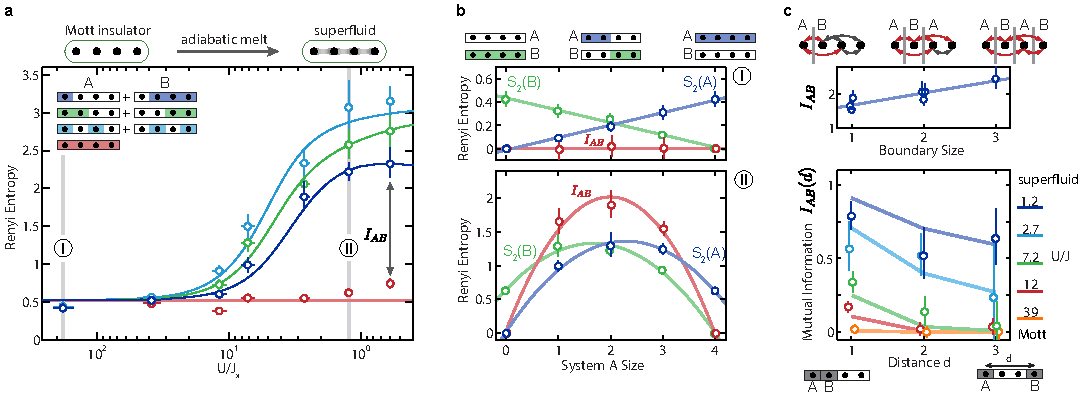
\includegraphics[width=\columnwidth]{figures/ch3/sf_mi_data/fig5.pdf} 
		\caption{\textbf{Measured Entropy in the MI to SF transition,}   }
		\label{fig:sf_mi_fig}	
\end{figure}


The SF to MI transition doesn't seem to have this. But why?! Well, it seems it has to do with the fact that the correlations in the ground state are really quite small. In our case, it is completely swamped by the correlations that arise from a conservation rule in our systme

\section{Ising model phase transition}

This section will start with a brief overview of another canonical phase transition in the Ising model with both longitudinal and transverse magnetic fields. Importantly, the implementation of this model in our Bose-hubbard model will have behavior that is more akin to the celebrated phase transition behavior expected without any conservation rules for equilibrium systems. Through the use of our DMD, we can access the full-counting statistics of the quantum state in the Fock basis. This allows us to directly probe the order parameter of the quantum phase, the single-site entropy, and the reversibility of the transition which probes its overall purity.

This model has been previously realized in this same experimental apparatus (cite paper) and is more thoroughly discussed in the following theses (cite waseem and alex ma).  The mapping from the Bose-hubbard model to a spin model was first proposed by Sachdev et. al (cite sachdev) and is accomplished my working in a reduced Hilbert space via a strong potential gradient in the optical lattice. The primary ingredients of this mapping are shown in Fig.~\ref{fig:IsingMap}.

This mapping starts in a regime where $U\gg J$ and $U/2<E<U$\footnote{The lower bound forgoes the contribution of second-order hopping processes that incorporate states outside of the prescribed basis for a faithful mapping to the Ising model. This was found to be a necessary step since these second-order processes provided a non-negligible fraction of population evolved into these states.}. This realizes a set of eigenstates that are approximately described by the Fock basis. The gradient potential, $E$, is then increased till $E>U$. This ramp will have brought site on-resonance with its neighbor. However, the celebrated dynamics of this transition arise from the collusion of all the particles in the system such that they transfer in a many-body coherent way.


$\tilde{t} = t/J$

$h_x = 2^{3/2}\tilde{t}$

$h_z = 1-\tilde{\Delta}$

$\tilde{Delta}=\Delta/J$

$\Delta = E-U$

$\delta_z^i = \delta E_i /J$

Transition happens at $E=U+1.85 t$ or $h_z = 1 - 0.66 h_x$

\begin{equation}
\label{eqn:isingHam}
H=J \sum_i S^i_z S^{i+1}_z - (h_z + \delta^i_z)S^i_z - h_x S^i_x
\end{equation}

\begin{figure}[h!]
		\includegraphics[width=\columnwidth]{figures/ch3/ising_data/IsingFig1.pdf} 
		\caption{\textbf{Measured Entropy in the MI to SF transition,}   }
		\label{fig:sf_mi_fig}	
\end{figure}


(we also get this same conservation rule but it arises as some sort of frustration in the ground state on the AFM side)
